\chapter{Theoretische Grundlagen  der Wegfindung}
	\label{Theorie}
\section{Modellierung der Anlagentopologie}
	\label{Graph_Anlage}
	Zur Berechnung eines Weges innerhalb der Anlage wird zunächst die Topologie der besagten Anlage benötigt. Für die Funktionsweise der \ac{FTF} wurde definiert, dass sich alle Fahrzeuge mittels optischer Merkmale auf einer definierten Teilstrecke bewegen. Zudem soll es den Fahrzeugen nur an festgelegten Entscheidungspunkten möglich sein, ihren Fahrzustand zu ändern und eine andere Teilstrecke auszuwählen. Dies bedeutet, dass alle Fahrzeuge, sobald sie sich für eine Teilstrecke entschieden haben, dieser bis zum nächsten Entscheidungspunkt folgen. Auf Basis einer solchen logischen Unterteilung der Anlage in Entscheidungspunkte und Teilstrecken als Verbindungen zwischen zwei Punkten, liegt es nahe, als Datenstruktur für die Modellierung der Anlagentopologie einen Graphen zu verwenden. Die Entscheidungspunkte entsprechen hierbei den Knoten, die korrespondierenden Teilwegstrecken stellen die Kanten des Graphen dar, mit beispielsweise dem Abstand als Gewichtung. Da sich die \ac{FTF} möglichst frei durch die Produktion bewegen sollen, wird als Grundform der Anlage ein ungerichteter Graph zur Abbildung der Topologie verwendet, jedoch soll es für die spätere Wegberechnung unerheblich sein, um welche Art von Graphen es sich handelt. Abbildung \ref{GraphenUebersicht} zeigt den Unterschied zwischen gerichteten und ungerichteten Graphen. Bei einem gerichteten Graphen kann ein Nachbarknoten nur entlang der angegebenen Kantenrichtung erreicht werden, bei ungerichteten Graphen ist ein Nachbarknoten über jede Verbindungskante erreichbar.

	\begin{figure}
		\centering
		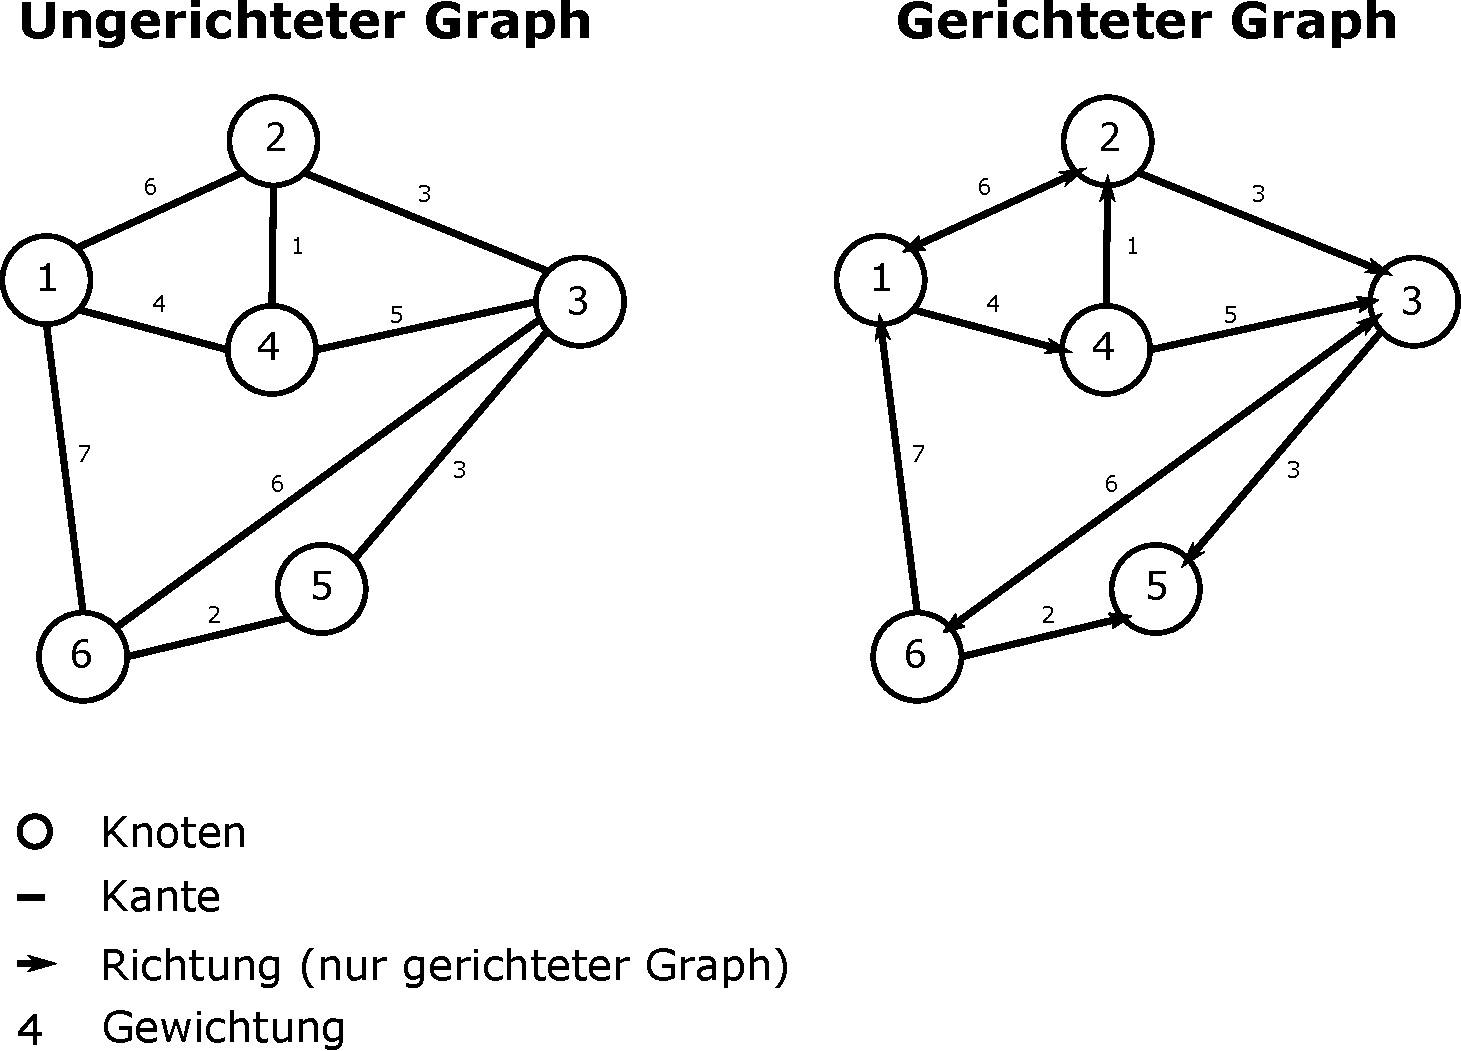
\includegraphics[scale=0.6]{/Bilder/UebersichtGraphenPDF}
		\vspace{0.2cm}
		\caption{Beispiel für ungerichtete und gerichtete Graphen mit Kantengewichten.}\label{GraphenUebersicht}
	\end{figure}

	Da der Graph die Abbildung einer realen Anlage ist, kann zudem ausgeschlossen werden, dass die Gewichtung der Kanten negativ ist, da dies je nach Art der Gewichtung nur wenig Nutzen bringen würde. Es existieren beispielsweise keine negativen Streckenabstände oder Fahrzeiten, die eine spezielle Betrachtung erforderlich machen und somit die Wahl der Wegfindungsalgorithmen einschränken würden.
	
\section{Auswahl der Algorithmen}

	Es existieren mehrere Algorithmen, welche sich mit der Problemstellung der Berechnung eines kürzesten Pfads zwischen zwei Knoten eines gewichteten Graphen befassen. Um eine passende Vorgehensweise auswählen zu können muss zuerst definiert werden, welche Kriterien ein potentieller Wegfindungsalgorithmus erfüllen muss.
	
	\subsection{Auswahlkriterien}
		\label{Kriterien_Alg}
		Für ein geeignetes Wegfindungssystem müssen die folgenden Aspekte berücksichtigt werden:
		\begin{enumerate}
			\item Die Berechnung soll auf einer \ac{SPS} des niedrigen Leistungssegments durchgeführt werden. Somit müssen die daraus resultierenden Beschränkungen bezüglich Komplexität und Speicherbedarf erfüllt sein.
			\item Eine \ac{SPS} ist ein Echtzeitsystem, welches das Programm zyklisch abarbeitet. Gleichzeitig wird auf der Steuerung auch die Fahraufgabe realisiert. Dadurch muss die Rechenzeit kurz genug sein, um eine Reaktionsfähigkeit des Fahrprogramms sicherstellen zu können.
			\item Die Wegfindung soll während der Ausführung eines vorausberechneten Fahrauftrags auf andere Fahrzeuge oder Änderungen der Anlagentopologie reagieren können.
			\item Es soll ein optimaler Weg gefunden werden. Optimal bedeutet im vorliegenden Fall einen möglichst kurzen Weg zum Zielknoten.
			\item Die Anlage soll gleichmäßig ausgelastet sein in Bezug auf Bearbeitungsstationen mit gleicher Funktionalität.
		\end{enumerate}
		
		Eine \ac{SPS}, wie sie in Punkt 1 beschrieben wird, erlaubt nur eine geringe Schachtelungstiefe der Unterprogrammaufrufe. Die verwendeten Steuerungen der S7-1200er Reihe erlauben beispielsweise eine Schachtelungstiefe von maximal 16 Bausteinaufrufen aus zyklischen und Anlauf-Bausteinen heraus \cite{S7-1200}.  Da diese kleinen \ac{SPS}en zudem über stark begrenzten Speicherplatz verfügen, muss bei einer Implementierung  mittels Stack überprüft werden, ob der hierfür statisch allozierte Speicherbereich auf der Steuerung zur Verfügung steht. Dies beschränkt den Einsatz von rekursiven Algorithmen jedoch auf Anwendungen, bei denen die Anzahl der Rekursionen von vornherein bekannt ist. Ein weiterer Nachteil von Rekursion ist, dass das Zeitverhalten von rekursiven Bausteinaufrufen nur schwer abschätzbar ist, und somit vorgegebene harte Echtzeitbedingungen des Systems verletzt werden können. Da die Anlagen aber beliebiger Art sein sollen, können Algorithmen die Rekursion verwenden somit nicht generell genutzt werden. Zudem fallen für die Implementierung diejenigen Algorithmen heraus, die nur sehr umständlich in der begrenzten Programmierumgebung für Echtzeitsteuerungen realisiert werden können.
		\\[4pt]
		Die Einhaltung der in Punkt 2 beschriebenen Echtzeitbedingung ist keine generelle Frage des Algorithmus sonder Sache der Implementierung. Hier müssen Programmteile mit Schleifenkonstrukten möglicherweise aufgebrochen und die Berechnung auf verschiedene Zyklen aufgeteilt werden.
		\\[4pt]
		Die in Punkt 3 erwähnte Reaktionsfähigkeit erfordert von den Algorithmen, dass sie auch in nur teilweise bekannten Umgebungen sicher einen Weg finden können. Für das Zusammenspiel ist eine Methode für die Vorhersage der Positionen anderer Fahrzeuge notwendig.
		\\[4pt]
		Da aus Gründen der Anlageneffizienz die Laufzeit eines Werkstücks durch die Anlage möglichst minimiert werden soll, wird von dem Wegfindungsalgorithmus gemäß Punkt 4 erwartet, dass er nicht nur schnell einen möglichen Weg findet, sondern dass der gefundene Weg auch der kürzeste, mit den begrenzten Anlageninformationen\footnote{ Abschnitt \ref{Zeitproblem} erläutert, dass Bewegungen anderer Fahrzeuge nur begrenzt vorausberechnet werden können.} berechenbare, Pfad zum Zielknoten ist.
		\\[4pt]
		Da die im Punkt 5 erwähnte gleichmäßige Auslastung mehr mit der Auswahl des geeigneten Zielknotens als mit der eigentlichen Wegfindung zu tun hat, ist diese Anforderung nur begrenzt für die Auswahl der Algorithmen von Bedeutung.
		
	\subsection{Betrachtete Algorithmen}
		\label{Betrachtete_Algorithmen}
		Im Angesicht der in \ref{Kriterien_Alg} ermittelten Auswahlkriterien wurden die folgenden Algorithmen näher betrachtet:
		
		\begin{longtable}{p{2.5cm} p{10cm}}
			
			\textbf{Dijkstra :} & Einer der Grundalgorithmen für das Kürzeste-Pfad-Problem, bei dem auch die kürzesten Entfernungen aller Knoten zu einem Startknoten ermittelt werden können.\\[0.5cm]
			\textbf{A* :} & Eine Abwandlung des Dijkstra-Algorithmus, bei dem die Anzahl der betrachteten Knoten verringert werden kann, indem Zusatzinformationen in Form einer Heuristik als Entscheidungshilfe für die Betrachtungsreihenfolge verwendet werden.\\[0.5cm]
			\textbf{\ac{MA*}\cite{Chakrabarti1989}:} &	Dieser Algorithmus beschränkt den Speicherverbrauch indem er den Topologiegraphen in Teilbäume unterteilt und nur erfolgversprechende Knoten und Teilgraphen im Speicher behält.\\[0.5cm]
			\textbf{\ac{RTA*}\cite{Korf1990}:} & Dieser Algorithmus unterteilt den Hauptalgorithmus in  Planungs- und Ausführungsphasen und beschränkt die Anzahl der betrachteten Knoten anhand einer Alpha-Beta-Suche. Durch diese Unterteilung kann ein gewisses Maß an Dynamik gewonnen werden, da der Algorithmus nach jeder Ausführungsphase die Restroute neu evaluiert und gegebenenfalls die aktuelle Route gegen einen neuen optimierten Weg ersetzt.\\[0.5cm]
			\textbf{\ac{D*}\cite{DStarAlg}\cite{Koenig2005}:} & Dieser Algorithmus wurde entwickelt für Topologien, welche nur teilweise bekannt sind, beziehungsweise die sich dynamisch verändern können. Zeiger, die entlang des jeweils kürzesten Weges vom aktuellen Knoten zum Startknoten zeigen, werden bei Anlagenänderung durch sogenannte "`Modify-Cost-Operationen"' ausgehend von der Anlagenänderung kaskadierend modifiziert, bis sich ein neuer statischer Zustand eingestellt hat. Die Wegberechnung nutzt diese Zeiger zur schnelleren Berechnung des kürzesten Pfades.\\[0.5cm]
			
		\end{longtable}
		
		Der Dijkstra-Algorithmus ist aufgrund seiner langen Berechnungszeit ungeeignet, für die Wegfindung im laufenden Betrieb der \ac{FTF} jedoch kann ausgenutzt werden, dass bei der Berechnung des kürzesten Pfades via Dijkstra die Abstände aller besuchten Knoten zum Startknoten ermittelt werden. Diese Abstände bilden die Basis zur Verbesserung der bei einem der anderen Algorithmen genutzten Heuristiken. Die Algorithmen \ac{MA*}, \ac{RTA*} und \ac{D*} sind alle Weiterentwicklungen des A*-Algorithmus. Die zu entwickelnde Modellanlage besitzt im vorliegenden Fall nur eine begrenzte Anzahl von Knoten. Dadurch ist der Nachteil des hohen Speicherbedarfs des Grundalgorithmus A* hier vernachlässigbar und der zusätzliche Aufwand für die Implementierung speichereffizienteren \ac{MA*}-Algorithmus kann zunächst vermieden  werden. Bei realen Anlagen mit einer höheren Anzahl an Knoten muss jedoch im Einzelfall betrachtet werden, ob eine Steuerung mit größerem Arbeitsspeicher oder die Implementierung des \ac{MA*}-Algorithmus notwendig ist. Der \ac{D*}-Algorithmus wurde wegen seiner höheren Komplexität und der Beschränkungen durch die Programmierumgebung nicht implementiert. Als zyklischer Wegfindungsalgorithmus wurde eine Mischform des A*-Algorithmus mit Planungs- und Ausführungsaspekten ähnlich denen von \ac{RTA*} verwendet, indem in regelmäßigen Abständen der bisher gefundene Teilweg verifiziert und bei Bedarf neu berechnet wird. Die verwendeten Algorithmen sollen nun etwas näher betrachtet werden.

\section{Gemeinsamkeiten der Algorithmen}

	Aufgrund der Tatsache, dass es sich bei dem A*-Algorithmus um eine Weiterentwicklung des Dijkstra-Algorithmus handelt, gibt es einige Grundprinzipien, die von beiden Algorithmen verwendet werden. Zum einen arbeiten beide mit einer Unterteilung der Graphenknoten in Unterklassen mit definierten Eigenschaften. Zum anderen wählen die Algorithmen den Knoten, der als nächstes betrachtet wird, nach bestimmten Kriterien aus. Bevor die Algorithmen einzeln vorgestellt werden, sollen zunächst ihre Gemeinsamkeiten dargestellt werden.
	
	\subsection{Klassifizierung der Knoten}
		\label{Klassifizierung}
		Um einen kürzesten Pfad zwischen zwei Knoten eines Graphen zu ermitteln, ist es hilfreich,während der Pfadberechnung alle Knoten des Graphen in drei Klassen aufzuteilen \cite{DijkstraAlg}:
		
		\begin{longtable}{p{2.5cm} p{10cm}}	
			\textbf{Klasse A:} & Die Menge aller Knoten, zu denen bereits ein kürzester Pfad  vom Startknoten aus bekannt ist. Diese Klasse wird auch als Closed-List bezeichnet.\\[0.25cm]
			\textbf{Klasse B:} & Die Menge aller Knoten, die mit mindestens einem Knoten aus Gruppe A verbunden sind, jedoch selbst nicht zu A gehören. Diese Klasse wird auch als Open-List bezeichnet.\\[0.25cm]
			\textbf{Klasse C:} & Die Menge der restlichen Knoten, die nicht in den Gruppen A oder B enthalten sind, und somit noch nicht betrachtet wurden.\\[0.25cm]
		\end{longtable}
		
		Analog können auch die Kanten des Graphen klassifiziert werden.
	
		\begin{longtable}{p{2.5cm} p{10cm}}
			\textbf{Klasse I:} & Die Menge aller Kanten, die in einem kürzesten Pfad zu einem der Knoten aus Gruppe A vorkommen.\\[0.25cm]
			\textbf{Klasse II:} & Die Menge aller Kanten, aus denen die nächste Kante für Gruppe I ausgewählt wird, wenn der korrespondierende Knoten aus B zur Gruppe A hinzugefügt wird. Es existiert immer genau eine derartige Kante für jeden Knoten aus Gruppe B. \\[0.25cm]
			\textbf{Klasse III:} & Die restlichen Kanten, die sich nicht in den Klassen I und II befinden.\\[0.25cm]
		\end{longtable}
		
		Eine derartige Einteilung der Knoten vereinfacht während der Berechnung des kürzesten Pfades die Entscheidung, welche Knoten momentan für die Wegfindung interessant sind und somit näher betrachtet werden sollten.
		
	\subsection{Auswahl des nächsten Knotens}
		\label{Abschaetz}
		Da nun die interessanten Knoten des Graphen identifiziert wurden, stellt sich die Frage in welcher Reihenfolge diese Knoten am besten betrachtet werden sollten.
		Diese Reihenfolge kann mittels einer Entscheidungsfunktion $f(n)$ bestimmt werden.
		
		\begin{itemize}
			\item \textit{Seien $s$, $n$ und $z$ beliebige Knoten des Graphen $G$, wobei $s$ der Startknoten und $z$ der Zielknoten für die Ermittlung des kürzesten Weges von $s$ zu $z$ sind.}\\
			\item \textit{Sei $f(n)$ die Summe der Kantengewichte eines kürzesten Pfades vom Knoten $s$ zum Knoten $z$, der zusätzlich den Knoten $n$ enthält.}
		\end{itemize}
		
		Es sei zunächst nicht bekannt, ob der Knoten $n$ auch auf dem kürzesten Pfad von $s$ nach $z$ liegt.
		Diese Entscheidungsfunktion, kann unterteilt werden in zwei Unterfunktionen $g(n)$ und $h(n)$ für die gilt \cite{Hart1968}:
		\begin{equation}
		f(n)=g(n)+h(n)
		\end{equation}
		
		Die Funktion $g(n)$ liefert hierbei den Wert des kürzesten Pfads vom Knoten $s$ zu $n$. Die Funktion $h(n)$ beschreibt den Wert eines kürzesten Pfades von $n$ zum Ziel $z$. A priori\footnote{also bevor der Wert von $f(n)$ bestimmt wurde.} sind die exakten Werte für $g(n)$ und $h(n)$ aber möglicherweise noch nicht bekannt. Somit werden für die Berechnung zunächst Schätzwerte für $g(n)$ und $h(n)$ verwendet. Sei also $\hat{g}(n)$ der Wert des bisher gefundenen kürzesten Pfades von $s$ nach $n$ und sei $\hat{h}(n)$ der mittels einer Heuristik geschätzte Wert des kürzesten Pfads von $n$ nach $z$. Somit kann der Wert von $f(n)$ geschätzt werden durch:
		\begin{equation}
			\hat{f}(n)=\hat{g}(n)+\hat{h}(n)
		\end{equation}
	
		Man geht zunächst davon aus, dass sich $n$ in der Klasse B befindet. $s$ befindet sich per Definition des Startknotens bereits in A, da die Entfernung von $s$ zu $s$ gleich null ist. Gemäß der Definition der Klasse B existiert somit mindestens ein Knoten $k_i$ aus der Klasse A, der durch eine Kante mit dem Knoten $n$ verbunden ist und für den $g(k_i)$ bereits bestimmt wurde\footnote{dies ist durch die Definition der Klasse A gegeben.}.
		\begin{itemize}
			\item \textit{Sei $M=\{k\in V(G),$ k ist direkter Nachbar von n$\} \cap A$}
			\item \textit{Sei $k_i=arg min\{v_{k,n},k\in M\}$}
		\end{itemize}
		 So gilt:
		%Sei $v_{k_i,n}$ die Gewichtung der Verbindungskante des Knotens $k_i$ nach $n$, so kann der exakte Wert für $g(n)$ wie folgt bestimmt werden:
		\begin{equation}
			g(n)=g(k_i)+v_{k_i,n}
		\end{equation}
		
		Dadurch kann der exakte Wert für $g(n)$ bestimmt werden. Die Kante mit der kleinsten Gewichtung, die den Knoten $n$ mit einem Knoten $k_i$ aus A verbindet, gehört zu der in Abschnitt \ref{Klassifizierung} definierten Klasse II.\\
		Es kann bewiesen werden \cite{Hart1968}, das die Wegfindungsalgorithmen immer den kürzesten Pfad von $s$ nach $z$ finden, sollte dieser existieren, wenn die Heuristik "`zulässig"' ist. Eine zulässige Heuristik, ist eine Schätzung deren Wert kleiner ist als der tatsächliche Wert, der geschätzt werden soll. Im vorliegenden Fall bedeutet dies, dass gelten muss:
		\begin{equation}
			\hat{h}(n)\le h(n).
		\end{equation}
		
		Dies hat zur Folge, dass der kürzeste Pfad von $s$ nach $z$ unter Verwendung einer solchen Heuristik $\hat{h}(n)$ bei Beendigung des Algorithmus nur aus Knoten der Klasse A besteht, also keine anderer Pfad existiert, der kürzer ist als der gefundene. Durch Speicherung des jeweiligen Vorgängers des aktuellen Knotens kann nach Beendigung der Algorithmen der kürzeste Pfad konstruiert werden. 
		\\
		Der Dijkstra-Algorithmus stellt hier den Standardfall dar, bei dem $\hat{h}(n)=0$ angenommen wird. Im Bezug auf A* werden unterschiedliche Werte für die Heuristik in Abschnitt \ref{Heuristik} näher betrachtet.
	
\section{Dijkstra-Algorithmus}
	Der erste für die Wegfindung verwendeten Algorithmus ist wie bereits erwähnt, der nach seinem Erfinder benannte Dijkstra-Algorithmus, der den kürzesten Pfad zwischen einem Startknoten und einem Endknoten\footnote{oder allen anderen Knoten.} eines Graphen ermittelt. Er kann verwendet werden für beliebige positiv gewichtete, gerichtete oder ungerichtete Graphen. Da in Abschnitt \ref{Graph_Anlage} negative Kantengewichtungen ausgeschlossen wurden, lässt sich der Algorithmus ohne Abwandlung auf den Graphen der Anlagentopologie anwenden.
	\subsection{Grundprinzip}
		\label{Dijkstra_Alg}
		
		Der Algorithmus funktioniert wie folgt. Zu Beginn befinden sich alle Knoten und Kanten respektive in den Klassen C oder III, da sie noch nicht betrachtet wurden. Als erstes wird der Startknoten S zur Klasse A hinzugefügt, da ein kürzester Pfad vom Startknoten zu sich selbst mit der Entfernung null bekannt ist. Der Startknoten kann somit als geschlossen angesehen werden. Nun werden folgende Schritte solange wiederholt, bis der Zielknoten erreicht wurde:
		\begin{center}
			\begin{minipage}{0.8\linewidth}

				\begin{enumerate}
					\item Man betrachte alle Kanten \textit{e} die den soeben zu A hinzugefügten Knoten mit einem Knoten \textit{k} aus B oder C verbinden. 
					\begin{itemize}
						\item Gehört \textit{k} bereits zur Gruppe B, so wird untersucht ob die Kante \textit{e} zu einem kürzeren Pfad zu \textit{k} führt, als der bisher gefundene kürzeste Pfad. Ist dies der Fall, so ersetzt \textit{e} die korrespondierende Kante aus II. Die Kante die durch \textit{e} ersetzt wird, wird wieder zur Gruppe III hinzugefügt.
						\item Gehört \textit{k} zur Gruppe  C, so wird \textit{k} zu B und \textit{e} zu II hinzugefügt.
					\end{itemize}
					\item Es wird die in Abschnitt \ref{Abschaetz} vorgestellte Funktion $f(n)$ verwendet, um genau den Knoten $b_i$ in der Klasse B zu finden, der den kleinsten Wert für $f(b_i)$ besitzt. Da bei dem Dijkstra-Algorithmus $\hat{h}(n)$ gleich Null ist, wird genau der Knoten  $b_i$ ausgewählt, für den $g(b_i)$ den kleinsten Wert hat, der also von den offenen Knoten den kleinsten Abstand zum Startknoten hat. Die zu $b_i$ gehörende Kante  aus II wechselt damit in die Klasse I.
				\end{enumerate}
				
			\end{minipage}
		\end{center}
	\subsection{Darstellung der Funktionsweise}
		Im Folgenden soll kurz die Funktionsweise des Algorithmus an einem einfachen Beispielgraphen mit vier Knoten gezeigt werden. Es soll der kürzeste Weg von Knoten 1 zu Knoten 3 gefunden werden.\\[4pt]
		Im ersten Schritt wird der Startknoten geschlossen, da dieser sich zu Beginn des Algorithmus als einziger Knoten in der Open-List befindet. Für alle Nachbarknoten muss nun die Länge der kürzesten Route zum Startknoten bestimmt werden. Dieser Wert entspricht genau dem Wert $g(n)$, wenn $n$ den jeweiligen Knoten bezeichnet. Die beiden Nachbarn des Startknotens, Knoten 2 und Knoten 4, werden zur offenen Liste hinzugefügt und ihre $g$-Werte berechnet. In Abbildung \ref{Dijkstra1} wird dies durch die roten Zahlen neben den entsprechenden Knoten dargestellt. Da bisher nur der Startknoten geschlossen wurde entsprechen die kürzesten Wege den Kantengewichtungen der jeweiligen Verbindungskanten vom Startknoten zu 2 und 4. Der Vorgängerknoten entlang des kürzesten Pfades wird durch einen roten Pfeil markiert:
		
		\begin{figure}[H]
			\centering
			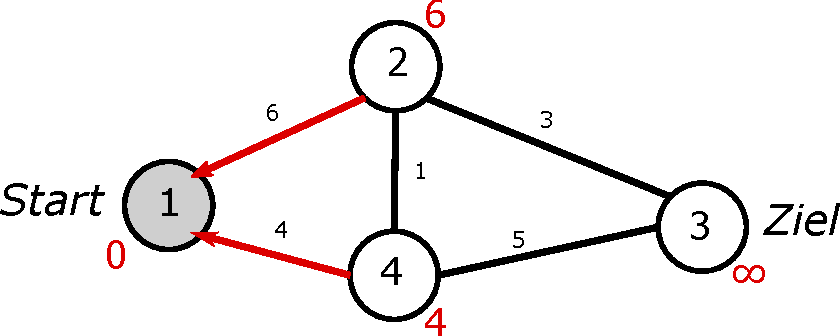
\includegraphics[scale=0.7]{/Bilder/Dijkstra1PDF}
			\vspace{0.2cm}
			\caption{Erster Schritt des Dijkstra-Algorithmus: Notation der kürzesten Routen. }\label{Dijkstra1}
		\end{figure}
		
		Nachdem der Startknoten vollständig betrachtet wurde, wird als nächstes der Knoten 4 geschlossen, da dieser die kürzeste bisher gefundene Route besitzt. Diese folgt aus $\hat{f}(Knoten 4)=4+0=4$ mit der Bedingung $\hat{h}(Knoten 4) = 0$ aus Abschnitt \ref{Abschaetz} für den Dijkstra-Algorithmus. Dadurch wird der Nachbarknoten 3 zur offenen Liste hinzugefügt. Aufgrund der Verbindungskante zwischen den Knoten ist nun eine Route zum Ziel bekannt und kann neben dem Knoten 3 notiert werden. Da diese aber nicht zwingend die Kürzeste ist, muss der Algorithmus weiter ausgeführt werden. Zum Knoten 2 wurde durch updaten des Knotens eine kürzere Route gefunden, die den Knoten 4 enthält. Diese wird notiert und die Vorgängerpfeile werden wie in Abbildung \ref{Dijkstra2} dargestellt abgeändert:
		
		\begin{figure}[H]
			\centering
			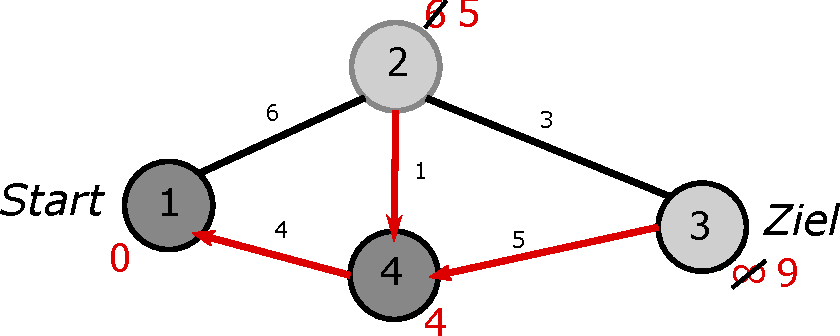
\includegraphics[scale=0.7]{/Bilder/Dijkstra2PDF}
			\vspace{0.2cm}
			\caption{Zweiter Schritt des Dijkstra-Algorithmus: Betrachten des Knotens mit dem bisherigen kürzesten Pfad. Update der anderen Knoten.}\label{Dijkstra2}
		\end{figure}
		
		Als nächstes wird Knoten 2 geschlossen, da der kürzeste Pfad zu 2 mit dem Wert 5 kleiner ist als der zum Zielknoten mit dem Wert 9. Dadurch wird ein neuer kürzester Pfad zum Ziel erkannt der den Knoten 2 enthält:
		
		\begin{figure}[H]
			\centering
			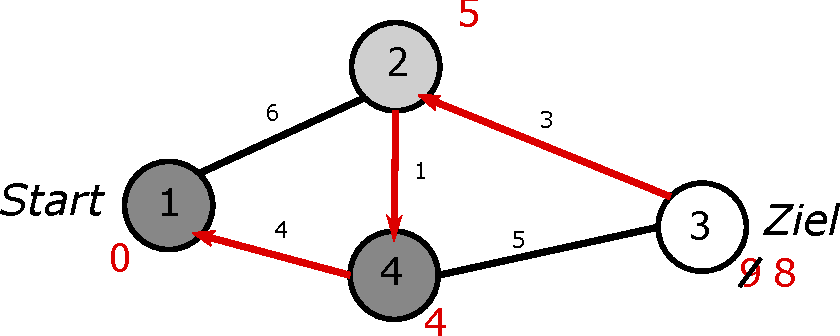
\includegraphics[scale=0.7]{/Bilder/Dijkstra3PDF}
			\vspace{0.2cm}
			\caption{Dritter Schritt des Dijkstra-Algorithmus: Expandieren des Knoten 2.}\label{Dijkstra3}
		\end{figure}
		
		Da nach dem Schließen von Knoten 2 nur noch der Zielknoten 3 in der offenen Liste übrig bleibt, kann dieser somit auch geschlossen werden. Wurde der Zielknoten zur Closed-List hinzugefügt, so beendet sich der Algorithmus und der kürzeste Pfad kann wie in Abbildung \ref{Dijkstra4} durch die Rückverfolgung  der Pfeile ausgehend vom Ziel bestimmt werden:
		
		\begin{figure}[H]
			\centering
			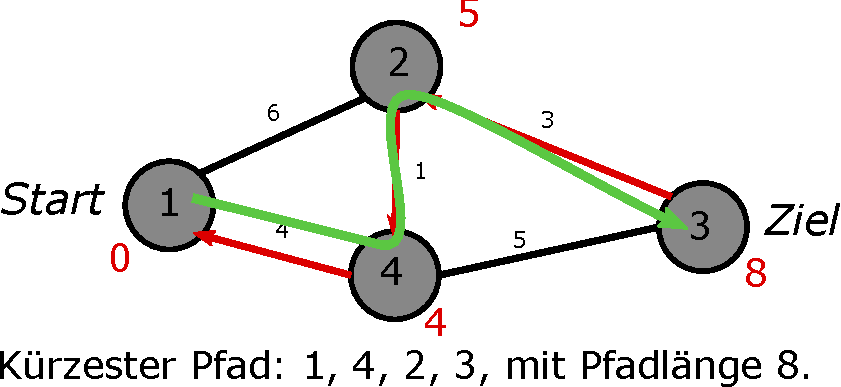
\includegraphics[scale=0.7]{/Bilder/Dijkstra4PDF}
			\vspace{0.2cm}
			\caption{Vierter Schritt des Dijkstra-Algorithmus: Rückverfolgung der Route nach Schließung des Zielknotens.}\label{Dijkstra4}
		\end{figure}
			
	\subsection{Berechnungsaufwand}
		Der Berechnungsaufwand des Dijkstra-Algorithmus beträgt in Landau-Notation vereinfacht $\mathcal{O}(\lvert \mathcal{V}\rvert ^2)$, beziehungsweise $\mathcal{O}(\lvert \mathcal{V}\rvert  \log \lvert \mathcal{V}\rvert + \lvert \mathcal{E}\rvert) $ bei der Implementierung mittels Fibonacci-Heaps \cite{Fredman1984}, wobei  $\lvert \mathcal{V}\rvert$ gleich der Anzahl der Knoten  und $\lvert \mathcal{E}\rvert$ gleich der Anzahl der Kanten des Graphen ist. Diese Vereinfachung gilt jedoch nur, wenn die Anzahl der Kanten in der gleichen Größenordnung liegt wie die Anzahl der Knoten, also beispielsweise nicht für vollständige Graphen, für die gilt $\lvert \mathcal{E}\rvert =\mathcal{O}(\lvert \mathcal{V}\rvert ^2)$.
	
\section{A*-Algorithmus}
	Der zweite verwendete Algorithmus für die Wegfindung ist der sogenannte A*-Algorithmus. Dieser ist eine Weiterentwicklung des in Abschnitt \ref{Dijkstra_Alg} vorgestellten Dijkstra-Algorithmus. Der grundlegende Unterschied ist jedoch, dass bei A* eine andere Bewertung der Betrachtungsreihenfolge von Knoten bei der Berechnung verwendet werden. Dies bedeutet, dass diejenigen Knoten und Kanten zuerst expandiert werden, bei denen die Wahrscheinlichkeit höher ist, dass sie Teil des kürzesten Pfades zum Zielknoten sind. Im Vergleich dazu wurde beim Dijkstra-Algorithmus immer genau der Knoten aus B als nächstes expandiert, der den kürzesten Abstand zu dem Startknoten hatte. Die Abbildung \ref{DijkstraVsA*} zeigt den Einfluss der Entscheidungsfunktion $f(n)$ bei der Auswahl des ersten betrachteten Knotens. Bei dem Dijkstra-Algorithmus wird zuerst Rosenheim betrachtet, da $\hat{f}(Rosenheim)=67km<\hat{f}(Ingolstadt)=78km$ ist. Der Dijkstra-Algorithmus berücksichtigt somit nicht, dass Ingolstadt näher am Ziel Regensburg liegt und somit der kürzeste Pfad wahrscheinlich über Ingolstadt verläuft. Beim A*-Algorithmus wird diese Zusatzinformation in Form der Heuristik-Funktion $h$ berücksichtigt. In diesem Beispiel wurde für die Heuristik der Luftlinienabstand zum Ziel gewählt \cite{Luftlinie}.
	
	\begin{figure}[h]
		\centering
		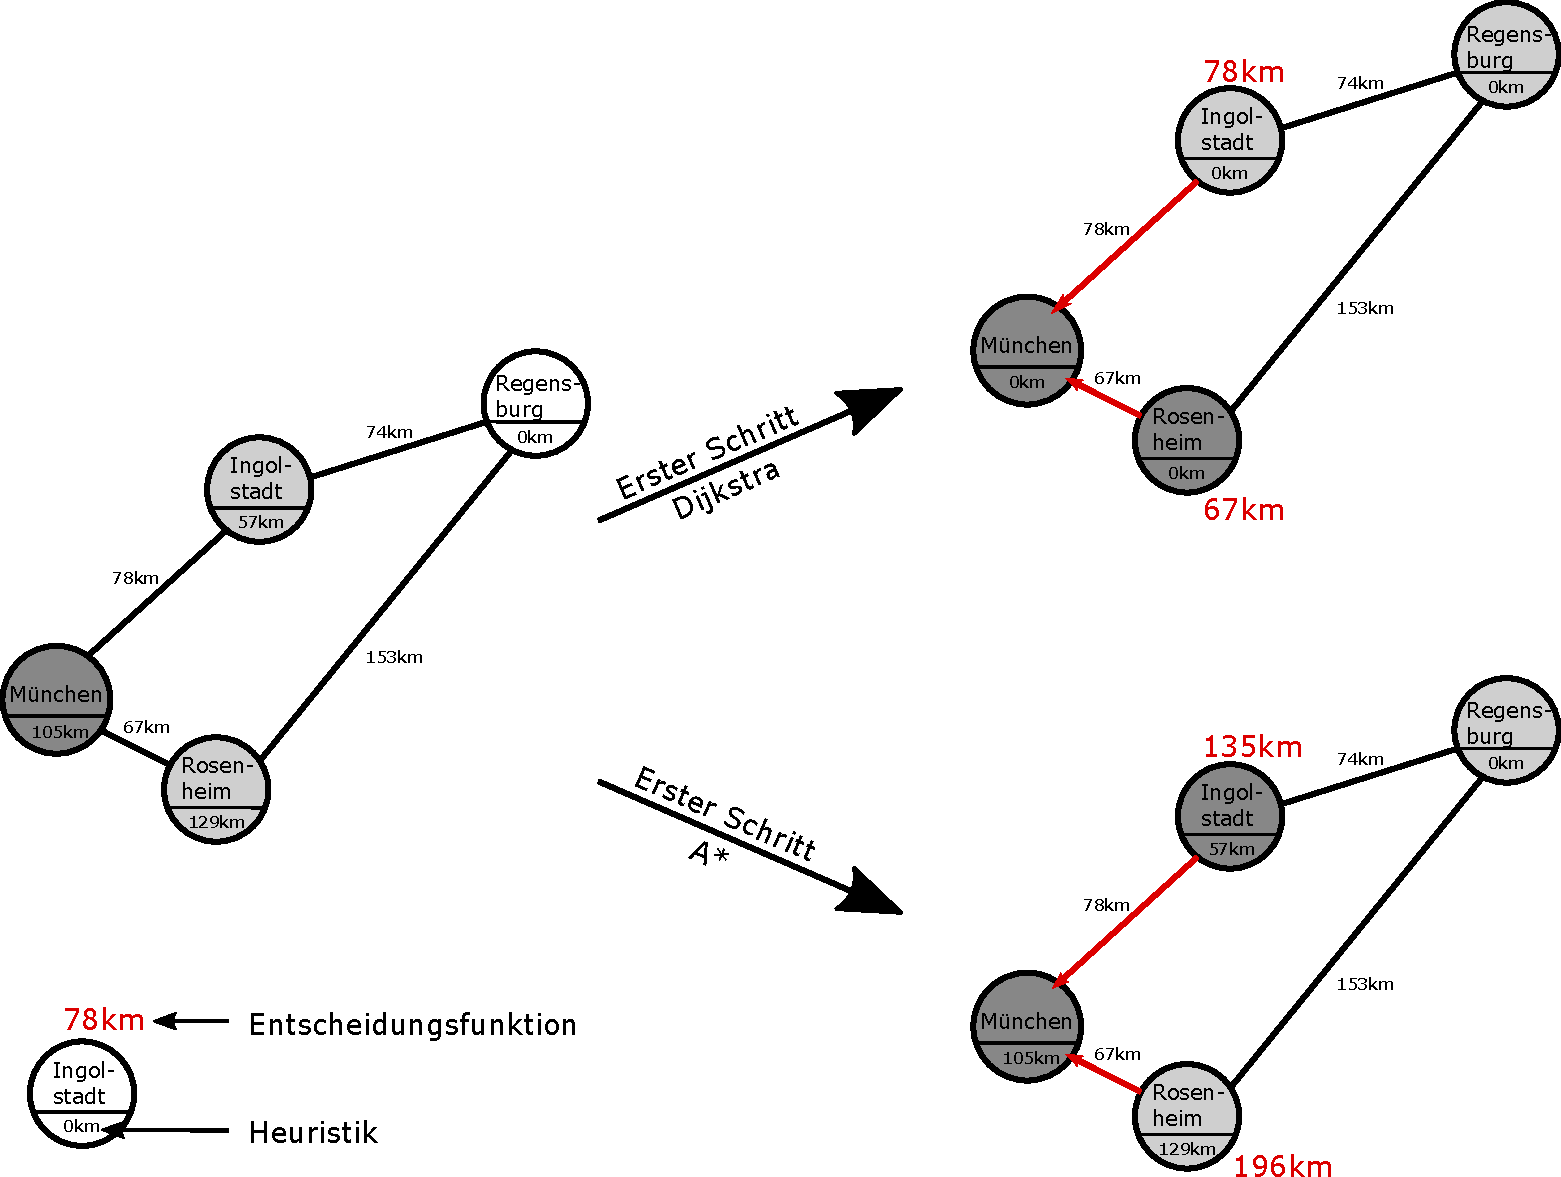
\includegraphics[scale=0.5]{/Bilder/DijkstraVsAStarPDF}
		\vspace{0.2cm}
		\caption{Vergleich des ersten betrachteten Knotens beim Dijkstra- und A*-Algorithmus am Beispiel des kürzesten Pfades von München nach Regensburg. Heuristik und Kantengewichte sind realen Weglängen gemäß \cite{Luftlinie}.} \label{DijkstraVsA*}
	\end{figure}
	Somit gilt hier:
	
	\begin{equation}
		\hat{f}(Ingolstadt)=g(Ingolstadt)+\hat{h}(Ingolstadt)=78km+57km=135km
	\end{equation}
	Der Wert der Entscheidungsfunktion kann für Rosenheim wie folgt bestimmt werden:
	\begin{equation}
		\hat{f}(Rosenheim)=g(Rosenheim)+\hat{h}(Rosenheim)=67km+129km=196km
	\end{equation}
	Aus diesem Grund wird zuerst Knoten Ingolstadt betrachtet, da $\hat{f}(Ingolstadt)<\hat{f}(Rosenheim)$ ist.
	
	
	Somit kann durch die zusätzlichen Informationen der Heuristik-Funktion eine Abschätzung der Wahrscheinlichkeit eines Knotens bezüglich seiner Zugehörigkeit zu dem  kürzesten Pfad vom Start zum Zielknoten gemacht werden. Mittels dieser Heuristik kann nun bereits vor Erreichen des Zielknotens eine Aussage über die voraussichtliche Länge der Route gemacht werden.
	
	\subsection{Grundprinzip}
		\label{A*-Alg}
		Die Funktionsweise des A*-Algorithmus kann als Erweiterung des Dijkstra-Algorithmus beschrieben werden \cite{Hart1968}. Unter Verwendung der in Abschnitt \ref{Abschaetz} definierten Entscheidungsfunktion kann wie folgt verfahren werden:
		
		\begin{itemize}
			 \item 	$s$, $z$ und $n$ sind Knoten eines Graphen. Es soll der kürzeste Pfad von $s$ nach $z$ ermittelt werden. 
			
		\end{itemize}
		
		\begin{center}
			
			\begin{minipage}{0.8\linewidth}
				
				
				\begin{enumerate}
					\item Man markiere $s$ als "`offen"' und berechne $f(s)$.
					\item Man wähle für $n$ denjenigen Knoten aus der Open-List aus, der den  kleinsten Wert für $f(n)$ besitzt.
					\item Falls $n=z$, wird $n$ als "`geschlossen"' markiert und der Algorithmus beendet.
					\item Andernfalls markiere man $n$ als "`geschlossen"' und füge alle von $n$ über maximal eine Kante erreichbaren Knoten $n'$ zur Liste der offenen Knoten hinzu, die noch nicht als geschlossen markiert wurden und berechne $f(n')$. 	Man springe zurück zu Schritt 2.
				\end{enumerate}
			\end{minipage}
		\end{center}
		
		Anhand dieser Vorgehensweise ist zu erkennen, dass bei dem A*-Algorithmus diejenigen Knoten bevorzugt betrachtet werden, die durch die Entscheidungsfunktion als "`wahrscheinlicher zum Ziel führend"' bewertet wurden, da anders als bei Dijkstra die Heuristik $\hat{h}(n)$ bei der Berechnung von $f(n)$ einen Einfluss auf das Ergebnis hat. Somit ist es sinnvoll diesen Bewertungsvorgang näher zu betrachten. 
		
	\subsection{Vergleich verschiedener Heuristiken h(n)}
		\label{Heuristik}
		Die in Kapitel \ref{Abschaetz} besprochene Entscheidungsfunktion $f(n)$ und diesbezüglich vor allem auch der Wert von $\hat{h}(n)$ haben einen großen Einfluss auf das Verhalten des A*-Algorithmus.
		Zur Veranschaulichung sollen einige Möglichkeiten für diese Heuristik betrachtet werden \cite{Patel2016}:
		\begin{enumerate}
			\item \textbf{$\hat{h}(n)=0$:} Wenn der Wert der Heuristik konstant auf Null gesetzt wird, so ist dies damit gleich zu setzen, als würden keine Zusatzinformationen zur Berechnung der Route verwendet. Dies bedeutet, dass immer genau der Knoten aus der Menge von offenen Punkten ausgewählt wird, dessen Abstand zum Startknoten am kleinsten ist. Der kürzeste gefundene Pfad durch einen Zwischenknoten $n$ hat zu jedem Zeitpunkt $i$ immer $f_i(n)=g_i(n)$. Somit entspricht der A*-Algorithmus mit der Heuristik $\hat{h}(n)=0$ genau dem Dijkstra-Algorithmus aus \ref{Dijkstra_Alg}.
			
			\item \textbf{$\hat{h}(n)<h(n)$:} Wenn der Abstand eines Knotens $n$ zum Ziel immer unterschätzt wird, also immer kleiner ist als der tatsächliche Abstand, so findet der A*-Algorithmus, wie bereits im Abschnitt \ref{Abschaetz} gezeigt, garantiert den kürzesten Pfad zwischen Start und Ziel. Je kleiner $\hat{h}(n)$ im Verhältnis zu $h(n)$ ist, desto mehr Knoten muss A* expandieren und umso langsamer läuft der Algorithmus.
			
			\item \textbf{$\hat{h}(n)=h(n)$:} Wenn der geschätzte Abstand eines Knotens zum Ziel genau dem tatsächlichen Abstand entspricht, expandiert A* immer die minimale Anzahl von Knoten entlang des kürzesten Pfades. Das heißt, dass wenn der kürzeste Pfad sechs Knoten enthält, der A*-Algorithmus nur genau sechs Knoten expandiert bevor der Zielknoten geschlossen und somit der kürzeste Pfad gefunden wurde. Zudem ist der Wert von $f_k(n)$ für jeden Teilknoten $k$ auf dem kürzesten Pfad immer gleich dem exakten Wert des Abstands zwischen Start und Zielknoten.
			
			\item \textbf{$\hat{h}(n)>h(n)$:} Wenn der geschätzte Abstand eines Knotens größer ist als der tatsächliche Abstand zum Zielknoten, so kann nicht mit Bestimmtheit gesagt werden, dass kein kürzerer Pfad zu bereits geschlossenen Knoten existiert.  Somit müssten, um den möglicherweise existierenden tatsächlichen kürzesten Pfad zu finden, bereits geschlossene Knoten erneut geöffnet werden. Wird dies nicht getan, so kann der A*-Algorithmus zwar unter Umständen schneller einen Pfad vom Start zum Ziel finden, es ist aber nicht garantiert, dass es sich um den Kürzesten handelt.
			
			\item \textbf{$\hat{h}(n)\gg h(n)$} Wenn der Schätzwert der Heuristik viel größer ist als der tatsächliche Abstand zum Zielknoten, so ist die Entscheidungsfunktion $f(n)$ nur noch abhängig von $\hat{h}(n)$ und der Wert der anderen Funktion $g(n)$ kann vernachlässigt werden. Somit hängt die Reihenfolge der expandierten Knoten nur noch von den Werten der Heuristik der entsprechenden Knoten ab.
		\end{enumerate}
		 
		Anhand der vorgestellten Eigenschaften der Heuristik wird erkennbar, das der A*-Algorithmus durch die Modifizierung der Heuristikberechnung an die gegebenen Anforderungen anpassbar ist. Anstatt einer genauen, aber langsamen Pfadberechnung, kann auf Kosten der Genauigkeit auch schnell ein möglicherweise nicht optimaler Weg zum Ziel gefunden werden. Zudem kann durch perfektes Wissen der Topologie der Anlage in kürzester Zeit der kürzeste Weg ermittelt werden.
	
	\subsection{Darstellung der Funktionsweise}
		Anhand des Beispiels aus Abbildung \ref{DijkstraVsA*} soll jetzt die Funktionsweise des A*-Algorithmus dargestellt werden. Die Knoten des Graphen stellen die Städte dar, die Kanten spiegeln Verbindungen  durch Schnellstraßen oder Autobahnen wieder. Die Gewichtungen der Kanten ist in diesem Beispiel die wirkliche Entfernung der Städte gemäß \cite{Luftlinie}. Auch als Heuristik wurde hier die Entfernung in Luftlinie zwischen den jeweiligen Städten und der Zielstadt gemäß \cite{Luftlinie} gewählt. Da die Luftlinie immer kürzer\footnote{oder im Extremfall gleich lang.} ist als eine Straße zwischen den Städten und somit die Bedingung $\hat{h}(n)\le h(n)$ erfüllt ist, findet der A*-Algorithmus sicher den kürzesten Pfad zum Zielknoten. Die Heuristik ist für jeden Knoten im unteren Drittel  angegeben. Der Ausgangspunkt des Beispiels ist der erste Schritt des Algorithmus, der bereits in Abbildung \ref{DijkstraVsA*} dargestellt wurde:  
		
		\begin{figure}[H]
			\centering
			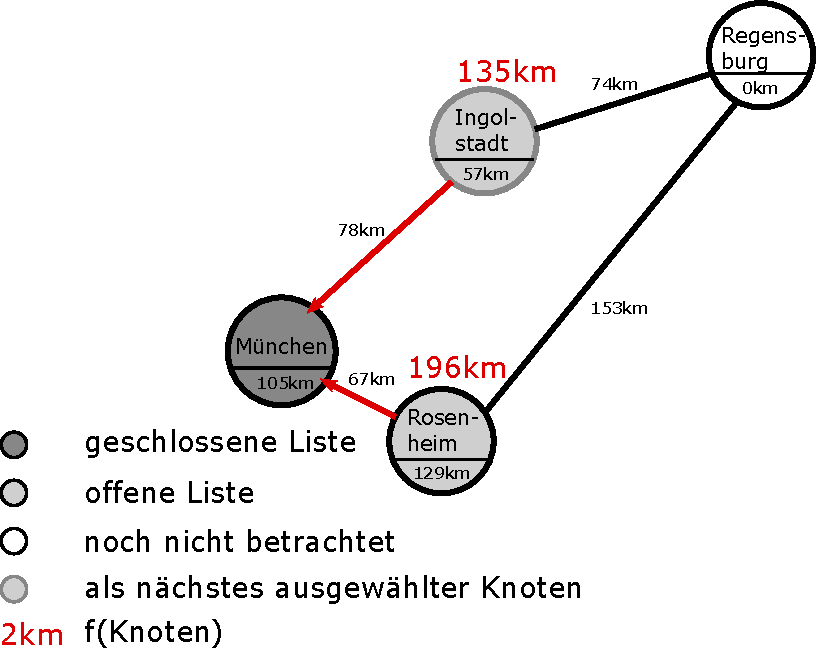
\includegraphics[scale=0.7]{/Bilder/AStar1PDF}
			\vspace{0.2cm}
			\caption{Erster Schritt des A*-Algorithmus: Betrachtung des Ersten Knotens.}
		\end{figure}
		
		Als nächster Knoten wird Ingolstadt geschlossen, da hier die Funktion $\hat{f}(n)$ den kleinsten Wert aller in der Open-List befindlichen Knoten hat. Im Anschluss wird $\hat{f}(Regensburg)$ bestimmt, um entscheiden zu können ob zuerst Rosenheim oder Regensburg expandiert werden muss. Da Regensburg von sich selbst 0km entfernt ist, hat die Entscheidungsfunktion $f(Regensburg)=g(Regensburg)$ den Wert $g(Ingolstadt)+74km=152km$:
		
		\begin{figure}[H]
			\centering
			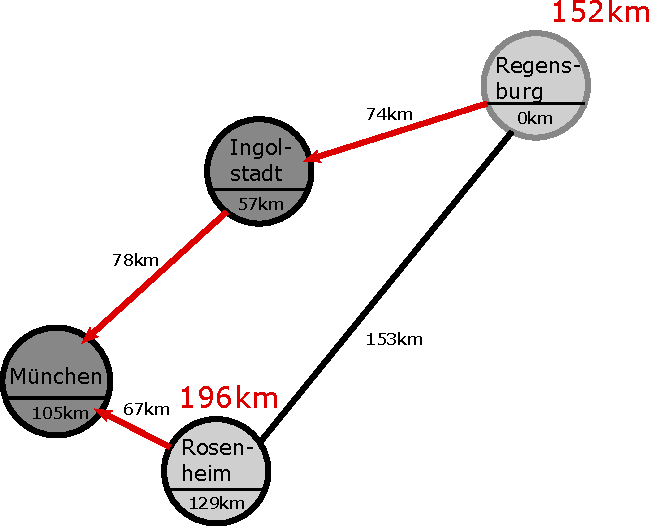
\includegraphics[scale=0.7]{/Bilder/AStar2PDF}
			\vspace{0.2cm}
			\caption{Zweiter Schritt des A*-Algorithmus: Hinzufügen von Regensburg zur Open-List.}
		\end{figure}
		
		Als nächstes wird der Knoten mit dem kleinsten Wert  für $\hat{f}(n)$ ausgewählt. Da $\hat{f}(Regensburg)<\hat{f}(Rosenheim)$ wird als nächstes der Knoten Regensburg geschlossen. Da Regensburg der Zielknoten ist beendet sich der Algorithmus. Da durch die Heuristik der Abstand zum Zielknoten immer unterschätzt wird ist $f(Rosenheim)$ sicher größer als $\hat{f}(Rosenheim)$. Es existiert somit sicher kein kürzerer Pfad nach Regensburg mehr als der bisher Gefundene:

		\begin{figure}[H]
			\centering
			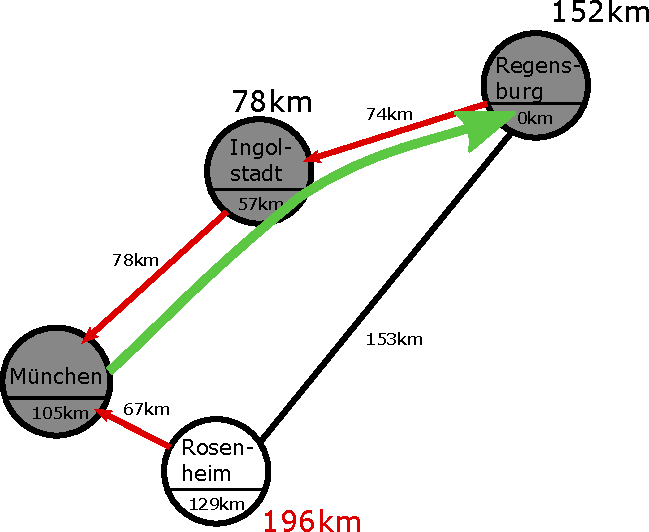
\includegraphics[scale=0.7]{/Bilder/AStar3PDF}
			\vspace{0.2cm}
			\caption{Dritter Schritt des A*-Algorithmus: Hinzufügen des Zielknotens zur Closed-List und Bestimmung des kürzesten Pfads} \label{A*3}
		\end{figure}
		
		Wie beim Dijkstra-Algorithmus kann nun durch Rückverfolgung der Vorgängerpfeile vom Ziel- zum Startknoten der kürzeste Pfad bestimmt werden. In Abbildung \ref{A*3} ist erkennbar, das der Knoten Rosenheim vom A*-Algorithmus nicht betrachtet wurde, obwohl er beim Dijkstra-Algorithmus in Abbildung \ref{DijkstraVsA*} als erster Knoten betrachtet wurde. Hierdurch ist erkennbar, dass je nach Qualität der Heuristik weniger Knoten betrachtet werden müssen, als dies bei Dijkstra der Fall wäre.
	
	\subsection{Berechnungsaufwand}
		\label{Aufwand_A*}
		Der Berechnungsaufwand für den A*-Algorithmus lässt sich nur schwer festlegen, da wie in \ref{Heuristik} beschrieben, die Berechnung des kürzesten Pfads sehr stark von der Heuristik abhängt. Unter der Annahme, dass auch wirklich der kürzeste Pfad gefunden wird, muss für die Heuristik gelten:
		\begin{equation} \label{eq:Heuristikbedingung}
			0\le \hat{h}(n)\le h(n)
		\end{equation}
		Somit muss auch der Berechnungsaufwand zwischen dem des Dijkstra-Algorithmus und dem Aufwand im Falle einer exakten Heuristik liegen. Da bei einer exakten Heuristik die Zahl der expandierten Knoten nur von der Anzahl der Knoten auf dem kürzesten Pfad abhängt, ist der Berechnungsaufwand konstant. Daraus folgt für eine beliebige Heuristik, die Bedingung \ref{eq:Heuristikbedingung} erfüllt:
		\begin{equation}
			\mathcal{O}(\lvert \mathcal{V}\rvert ^2)\ge \mathcal{O}(\hat{h}(n))\ge \mathcal{O}(\lvert \mathcal{V}\rvert)
		\end{equation}
		
		Somit ist der Berechnungsaufwand im schlechtesten Fall quadratisch, im besten Fall aber gleich der Anzahl der Knoten des kürzesten Pfads. Eine bessere Heuristik führt somit dazu, dass weniger Knoten als im schlechtesten Fall expandiert werden müssen und sich somit der Rechenaufwand verringert.
		
	\section{Zusammenspiel der Algorithmen}
		\label{Verwendung_Alg}
		Wie bereits in Abschnitt \ref{Betrachtete_Algorithmen} erwähnt, wird nun ausgenutzt, dass der Dijkstra-Algorithmus die Abstände vom Startknoten zu allen betrachteten Knoten ermittelt.  Der Nachteil, dass er vergleichsweise langsam arbeitet wird umgangen, indem der Algorithmus nicht in der zeitkritischen zyklischen Bearbeitungsphase sondern beim Hochfahren der CPU ausgeführt wird. Hier ist die Fahrzeugsteuerung\footnote{und vor allem auch der Watchdog-Timer} noch nicht aktiv und somit können auch längere Berechnungen ausgeführt werden. Zusätzlich werden nicht alle Knoten als Startknoten für die Abstandsberechnung mittels Dijkstra verwendet, sondern nur solche, die im späteren Anlagenbetrieb als endgültige Zielknoten für die Wegfindung infrage kommen. Als solche Zielknoten kommen vor allem die Knoten in Frage, an denen sich Maschinen befinden oder die eine spezielle Funktion erfüllen, wie beispielsweise der Anlagenausgang. Transitknoten, die nur im Verlaufe der Abarbeitung einer Route durchfahren werden, aber an denen nie eine Route endet, können hierbei ausgelassen werden.
		\\[4pt]
		Die Ergebnisse der Dijkstra-Berechnungen werden in einer Tabelle gesichert und als Basis für die Heuristik der Wegfindung mittels A* im zyklischen Betrieb verwendet. Wie in  Abschnitt \ref{Heuristik} gezeigt wurde, ist die Anzahl der expandierten Knoten und somit auch die Laufzeit minimal, wenn als Heuristik der exakte Abstand zum Ziel genutzt wird. Dieser Fall ist, unter der Bedingung das sich die Anlage seit dem Hochfahren der CPU nur geringfügig geändert hat, durch die Verwendung der Abstände des entsprechenden Ziels aus der Dijkstra-Tabelle gegeben. Auch bei Änderungen, wie beispielsweise Sperrungen von Kanten oder der Blockade von Teilstrecken durch andere Fahrzeuge, erfüllt diese Heuristik noch die Anforderung $\hat{h}(n)\le h(n)$, da die neue exakte Route sicher länger ist, als die vorausberechnete ideale Route ohne Hindernisse. Bei Hinzufügen neuer Kanten zur bestehenden Anlage muss die CPU neu gestartet werden\footnote{aus im Abschnitt \ref{Knotenliste} beschriebenen Gründen}, da hierdurch kürzere Wege entstehen könnten, welche die Bedingung aus Gleichung \ref{eq:Heuristikbedingung} verletzen würden.
		
		
				





